\chapter{Background}

\label{chap:Background}
This chapter introduces a brief overview of the major techniques and models used throughout the thesis. In particular, handshake circuits -- a specification formalism for synthesis of self-timed hardware; Petri nets -- a graph-based notation for reasoning about concurrent behaviour; conditional partial order graphs (CPOG) -- a versatile notation for describing a family of partial orders.


\section{Handshake circuits}


One of the approaches to design of asynchronous circuits is syntax-directed mapping with 
handshake circuits as an intermediate format. The parse tree of a program source code written in 
a CSP-style \cite{csp} language can be interpreted as a graph of components, connected with communication links
called handshake channels. The components can then be individually mapped to gate-level implementations
with complete circuit derived by implementing the handshake channels with wires.

This approach has been first used by Philips in their Tangram \cite{tangram} design tool
and later made publicly available after the similar free Balsa \cite{balsa} system has been released.

This thesis will be working with Balsa handshake components.

A handshake activation $h$ is said to \emph{enclose} a process $p$ if $p$ can only start after $h$ gets a request and $h$ can get an acknowledgement only after $p$ gets finished.

A \emph{handshake circuit} consists of handshake components which interact by request/acknowledgement handshaking 
over communication channels.
Each \emph{handshake component} is specified by a set of ports and a process communicating over those ports.
A \emph{protocol} is assigned to each port, which specifies whether the process initiates the handshakes
over an \emph{active port} or awaits for the other party over a \emph{passive port}. 
It also specifies the direction and size of data transferred during the handshakes.
Each \emph{channel} connects two ports of the same data size with one port being active and the other being passive.

On diagrams used in this thesis we display handshake components with large circles with a process symbol inside
and handshake ports with small circles where filled circle stands for active port and hollow circle stands for passive port.
Channels are displayed as lines between the corresponding ports with the direction of the arrow corresponding to the
direction of data flow.


The defining feature of a handshake component is the process associated with it. 
In Balsa there are about fifty types of processes with each 


\begin{itemize}
\item
Sequence is a component with three control ports: a passive port $s$ and two active ports $t_1$ and $t_2$.
The behaviour of the component is as follows: upon receiving an activation it encloses the two activations activation of $t_1$ action   awaits for activation over $s$ and encloses the following: a handshake over $activate_1$ followed by a handshake over $activate_2$; after receiving the acknowledgement  and acknowledges

\item
Concur is a component with a similar external interface: it has a passive port $activate$ and two active ports $activate_1$ and $activate_2$.
The behaviour during the activation on $activate$ is to activate $activate_1$ and $activate_2$ concurrently.

\item
Sync is a component with three control ports: two passive ports s_1 and s_2 and an active port t. 
This component ensures that $t$ is enclosed 
\end{itemize}



\begin{figure}
\centering
\subfloat[Sequence\label{fig:SequenceOptimised}]{
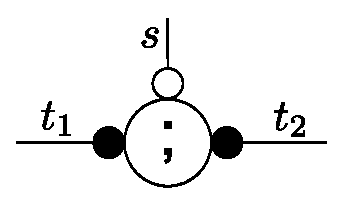
\includegraphics[scale=0.5]{figures/Control/sequence-HC}
} {}
\subfloat[Concur\label{fig:Concur}]{
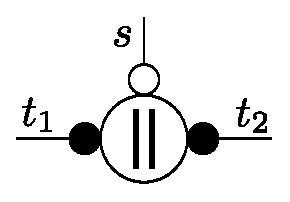
\includegraphics[scale=0.5]{figures/Control/concur-HC}
} {}
\subfloat[BinaryFunc\label{fig:BinaryFunc}]{
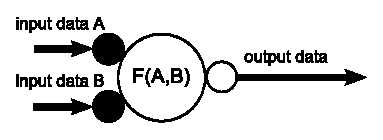
\includegraphics[scale=0.4]{figures/Data/binaryfunc-HC}
} {}
\subfloat[CallMux\label{fig:CallMux}]{
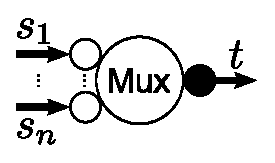
\includegraphics[scale=0.5]{figures/Data/callmux-HC}
} {}
\subfloat[Variable\label{fig:Variable}]{

\includegraphics[scale=0.5]{figures/Data/variable-HC}
} {}
\subfloat[While\label{fig:While}]{

\includegraphics[bb=0bp 0bp 134bp 80bp,scale=0.5]{figures/while-HC}
} {}
\subfloat[Case\label{fig:Case}]{

\includegraphics[scale=0.5]{figures/case-HC}
}

\caption{Handshake components}
\end{figure}





 Each channel connects two ports. Each port is connected to a channel. 
with which it
can be connected point-to-point to a port of another handshake circuit by means of a channel. 
. Each
channel carries request and acknowledgement signalling as well as an optional data payload. The
requests flow from the active component ports (filled circles) towards passive component ports
(open circles). Acknowledgements flow in the opposite direction to requests. Where a channel
carries data, the direction of the data is indicated by an arrow on that channel’s arc. The direction
of data may be different from the direction of signalling to support push and pull port and channels.
A handshake component can be activated by sending request to its passive port. When activated, 
it sends requests to a subset of its active ports and waits for acknowledgements. The
subset of the ports activated by the component is determined by its function and may be data-
dependent. The order in which the component activates its ports is shown by small numbers next
to the ports. The ports of a handshake component which are marked with the same number are ac-
tivated concurrently. When all activated ports are acknowledged, the handshake component sends
an acknowledgement to the passive port from which it was activated and finishes its operation until
the next activation.

\section{Improved Parallel Composition}\label{sec_intro}



\subsection{Abstract}
Parallel composition of labelled Petri nets is a fundamental operation in modular design. It is often used to combine models of subsystems into a model of the whole system.
Unfortunately, the standard definition of parallel composition almost always yields a `messy' Petri net, with many implicit places, causing performance deterioration in tools that are based on structural methods. In this paper we propose an optimised algorithm for computing the parallel composition. It often produces nets with fewer implicit places, which are thus better suited for subsequent application of structural methods.

\subsection{Introduction}

Parallel composition (\aka synchronous product) of labelled
Petri nets is a fundamental operation in modular design. It is
often used to combine models of subsystems into a model of the
whole system. In particular, there is a nice correspondence
between parallel composition of Signal Transition Graphs
(STGs), a class of labelled Petri nets used for modelling
asynchronous circuits, and connecting circuits by wires. Hence
performing this operation efficiently is important in practice.

Unfortunately, the standard definition of parallel composition almost always yields a `messy' Petri net, with many implicit places (even if the component Petri nets did not have them). Some of these places are easy to remove (\eg duplicate places, which have the same pre- and postsets), but in general for removing others one needs full-blown model checking, which is infeasible if the resulting composition is large.
Although implicit places do not have noticeable effect on tools based on state space exploration, such as \petrify~\cite{ckkly97}, the performance of tools that are based on structural methods, such as \desij~\cite{Sch07}, often deteriorates.

Consider an example shown in Fig.~\ref{fi-motivating-example1},
which shows the STG specifications of two components (a,b) and
the specification of the environment (c). (The used short-hand
drawing notation for STGs is explained in
Sect.~\ref{sec_pn_basic}.) The model of the behaviour of the
entire system can be obtained by constructing the parallel
composition of these three STGs, which is shown in part (d) of
this figure. One can see that it contains a few implicit places
(which are not duplicate places); intuitively, they appear due
to repeated causality specifications for every signal: the one
coming from the component where this signal is an output, and
others --- from the components where it is an input. Removing
these places yields a much `cleaner' STG, coinciding with that
shown in Fig.~\ref{fi-motivating-example2}(d).

\begin{figure}[!tb]
    \centering
    \begin{minipage}[b]{0.4\columnwidth}
    \centering
        $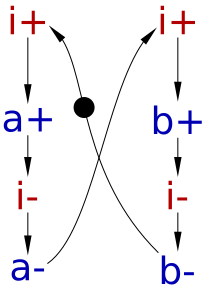
\includegraphics[scale=0.3]{EXPERIMENTS/stg/toggle}
        \atop
        \mbox{\rule[1.3em]{0em}{0em}(a) Toggle}$
        \\[0.5em]
        $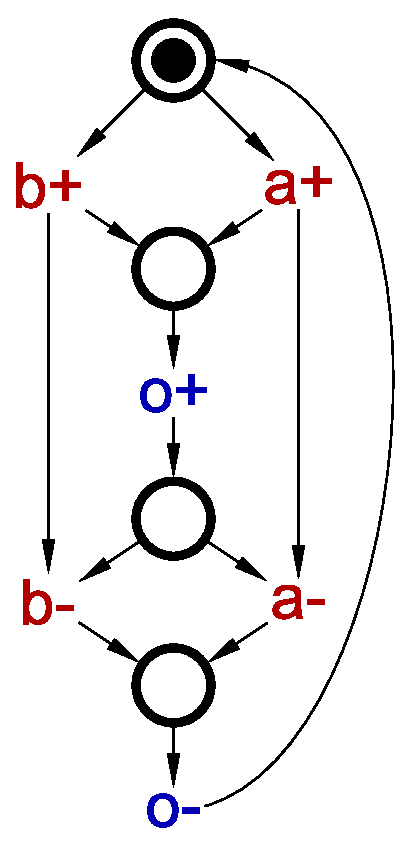
\includegraphics[scale=0.3]{EXPERIMENTS/stg/mix}
        \atop
        \mbox{\rule[1.3em]{0em}{0em}(b) Call}$
        \\[0.5em]
        $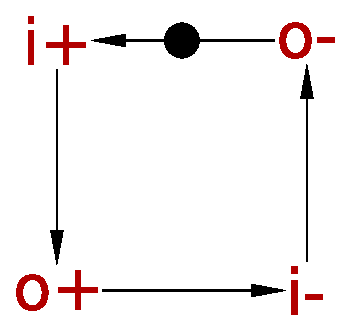
\includegraphics[scale=0.3]{EXPERIMENTS/stg/env}
        \atop
        \mbox{\rule[1.3em]{0em}{0em}(c) Environment}$
    \end{minipage}
    $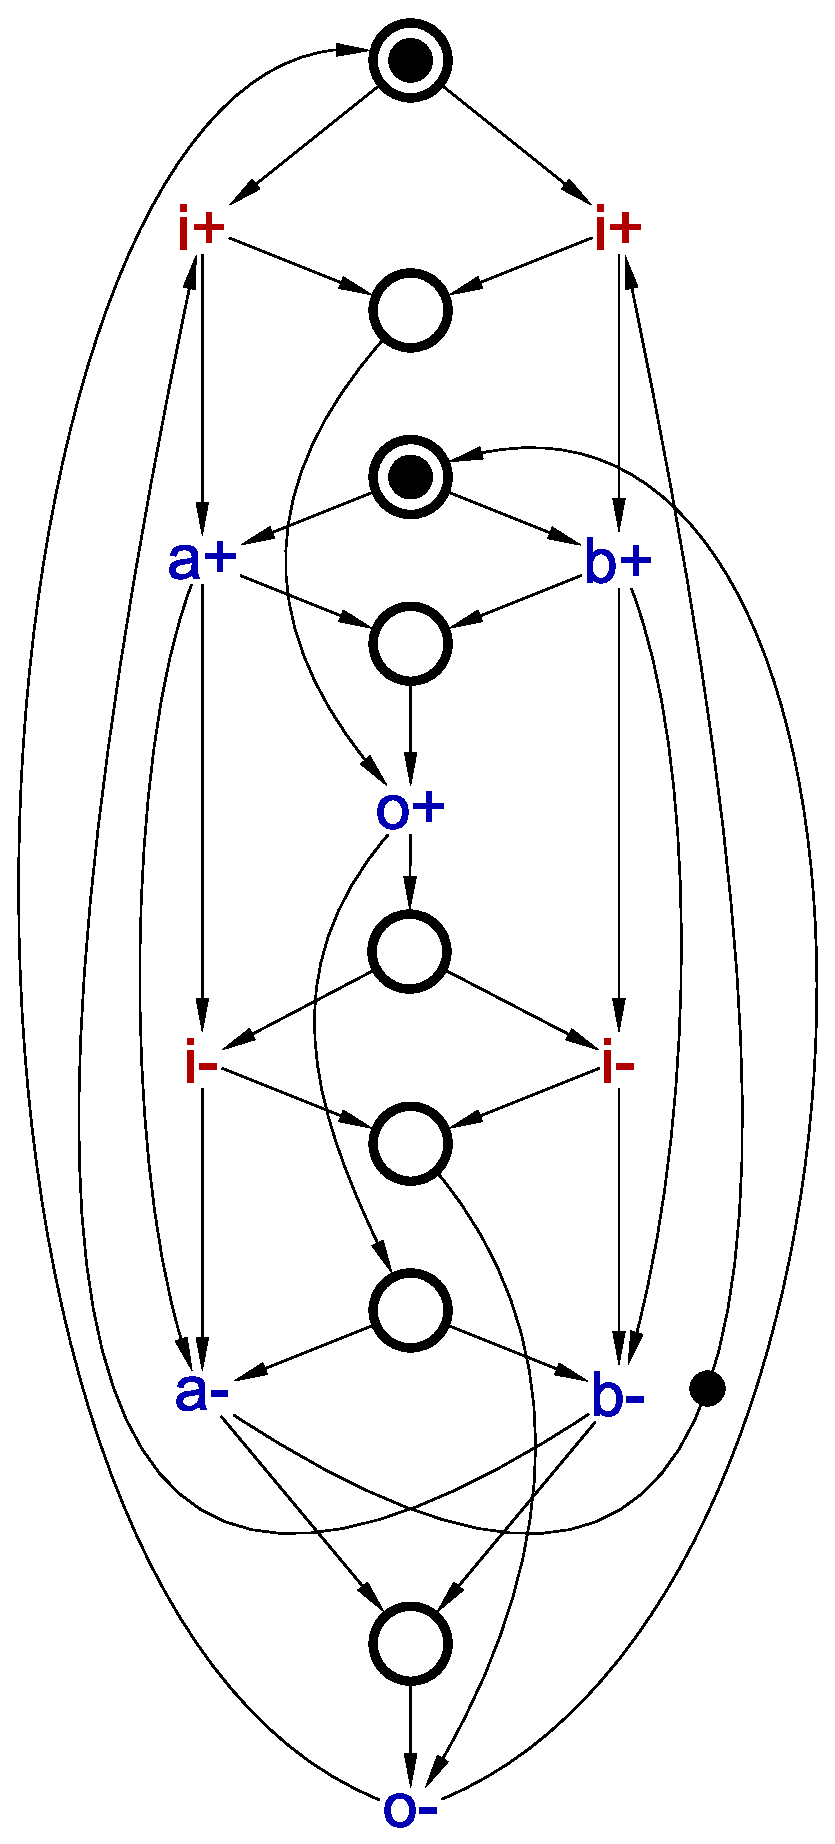
\includegraphics[scale=0.3]{EXPERIMENTS/stg/simple_standard}
    \atop
    \mbox{\rule[1.3em]{0em}{0em}(d) Composition}$
    \caption{\label{fi-motivating-example1}
        Example of standard STG composition.
    }
\end{figure}

\begin{figure}[!tb]
    \centering
    \begin{minipage}[b]{0.4\columnwidth}
        \centering
        $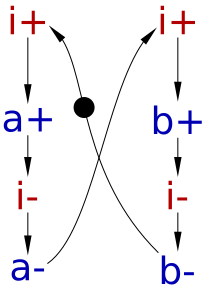
\includegraphics[scale=0.3]{EXPERIMENTS/stg/toggle_opt}
        \atop
        \mbox{\rule[1.3em]{0em}{0em}(a) Toggle}$
        \\[0.5em]
        $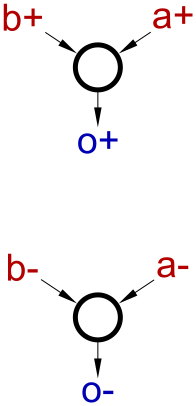
\includegraphics[scale=0.3]{EXPERIMENTS/stg/mix_opt}
        \atop
        \mbox{\rule[1.3em]{0em}{0em}(b) Call}$
        \\[0.5em]
        $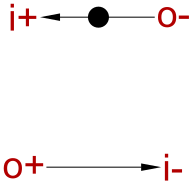
\includegraphics[scale=0.3]{EXPERIMENTS/stg/env_opt}
        \atop
        \mbox{\rule[1.3em]{0em}{0em}(c) Environment}$
    \end{minipage}
    $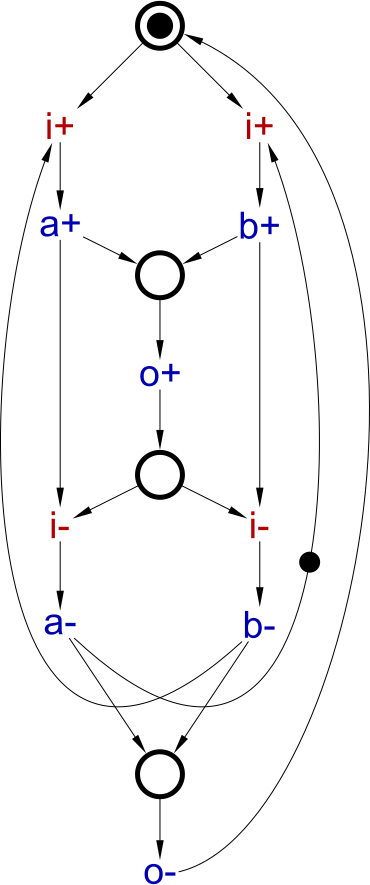
\includegraphics[scale=0.3]{EXPERIMENTS/stg/simple_improved}
    \atop
    \mbox{\rule[1.3em]{0em}{0em}(d) Composition}$
    \caption{\label{fi-motivating-example2}
        Example of improved STG composition: the components are obtained from the corresponding ones in Fig.~\ref{fi-motivating-example1} by removing some places, and then the standard parallel composition is applied to these modified components.
    }
\end{figure}


One operation where implicit places matter is \emph{transition contraction,}~\cite{vowo02lncs} which is a crucial part of the re-syn\-the\-sis approach~\cite{CN-02,KVL-96,PC-96}. The idea is to hide the internal communication between the components (by labelling the corresponding transitions as `dummy' --- they correspond to signals $a$ and $b$ in our example), contract as many of these dummy transitions as possible (whereby reducing the size of the STG), and re-synthesise the obtained STG as a circuit (which is often smaller than the original circuit due to removal of some signals). Transition contraction has to be performed on very large STGs (corresponding to the whole control path of the circuit), and so, for efficiency, it has to be a structural operation. Unfortunately, such structural contractions are not always possible (see Sect.~\ref{sec_pn_basic}), and implicit places in the preset and/or postset of a transition can prevent contracting it, even if a contraction is possible after removing these implicit places. In our example, \desij cannot contract any of the dummy transitions in the STG in Fig.~\ref{fi-motivating-example1}(d), even though it performs some structural tests for place redundancy; however, it is able to contract all the dummy transitions if the implicit places are removed, \ie when applied to the STG in Fig.~\ref{fi-motivating-example2}(d).

The main contribution of this paper is a new me\-thod for computing the parallel composition of labelled Petri nets, that generates fewer implicit places. It uses the \emph{freeness from computation interference (FCI)} assumption, stating that the situation when one component wants to produce an output, but is prevented from doing so by another component which is not ready to receive it, is impossible. Violation of FCI means that the behaviour of the composition does not correspond to that of the physical system. For example, an output of a circuit component cannot be physically disabled by another component that is not ready to receive this signal, and so producing this output will lead to malfunction; however, the composition will be oblivious to it, and behave as if such an output could not be produced.
Hence FCI is a basic correctness requirement --- if it is violated, there is no point in computing parallel composition, as its behaviour will not describe that of the physical system. In practice, FCI is often guaranteed by construction, \eg it is always guaranteed for the control path of a \balsa~\cite{EB-02} or \haste/\tangram~\cite{berkel91,haste-manual} specification of an asynchronous circuit. The idea of using the FCI condition is reminiscent of the method of input/output exposure in the synthesis by direct mapping described in~\cite{SBY-07}, and of the correct by construction composition of Petri nets for circuit components and the environment used in the \ditopn tool~\cite{JF-00}.

The main idea of the method we propose here is illustrated by the example in Fig.~\ref{fi-motivating-example2}. Before doing the parallel composition, one can remove some of the places in the components as shown in parts (a--c) of the figure and then compose the modified STGs. The precise conditions that allow to remove a particular place will be stated in Sect.~\ref{se-main}; at this point it is only important that they are structural and thus can be efficiently checked. This guarantees that the number of places in the resulting Petri net is smaller (as the number of places in the composition is the total number of places in all the components), and, under the FCI assumption, the resulting behaviour will be the same (in the sense of isomorphism of the reachability graphs). In particular, in our example, composing the modified components yields the STG in Fig.~\ref{fi-motivating-example2}(d), which in this case contains no implicit places. Observe that the modified components on their own can have rather bad behaviour and in particular can be non-implementable; however, it does not matter, as they are never used on their own, but only in composition with other components, and the resulting behaviour of the composition is guaranteed to correspond to that of the standard composition.

Re-synthesis of asynchronous circuits is the intended application of the proposed method. However, we envisage that it has a much wider applicability, as composition of labelled Petri nets is a fundamental operation, and the FCI assumption often holds in practice.

\section{Conditional Partial Order Graphs\label{sec:CPOG-model-essentials}}

A \emph{Conditional Partial Order Graph}~\cite{2009_mokhov_phd}\cite{2010_mokhov_ieee}
is a quintuple $H=(V,\ E,\ X,\ \rho,\ \phi)$, where $V$ is a finite
set of \emph{vertices}, $E\subseteq V\times V$ is a set of \emph{arcs}
between them, and $X$ is a finite set of \emph{operational}\emph{variables}. An \emph{opcode} is an assignment $(x_{1},\ x_{2},\ \dots,\ x_{|X|})\in\{0,\ 1\}^{|X|}$
of these variables; $X$ can be assigned only those opcodes which
satisfy the \emph{restriction function} $\rho$
of the graph, i.e. $\rho(x_{1},\ x_{2},\ \dots,\ x_{|X|})=1$. Function
$\phi$ assigns a Boolean \emph{condition} $\phi(z)$ to every vertex
and arc $z\in V\cup E$ of the graph.

\begin{figure}[h]
\hfill{}\subfloat[Full notation]{

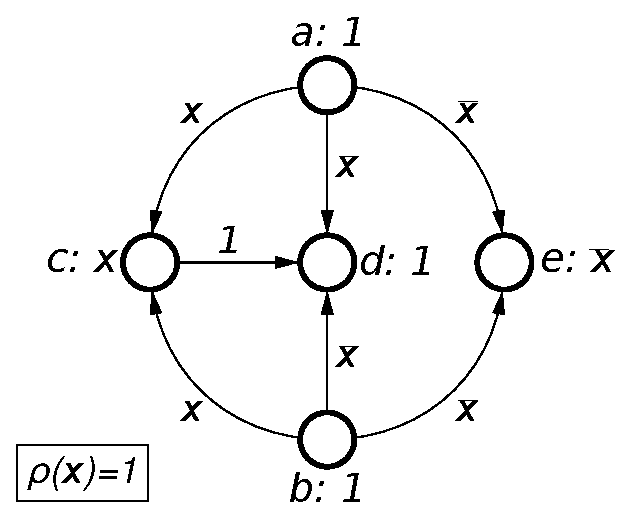
\includegraphics[scale=0.45]{fig/cpog}}\hfill{}\subfloat[Simplified notation]{

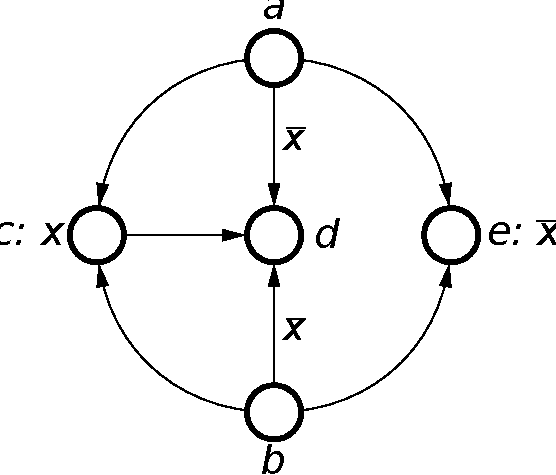
\includegraphics[scale=0.45]{fig/cpog_simplified}}\hfill{}

\begin{centering}
\subfloat[Multiple CPOG projections]{\begin{centering}
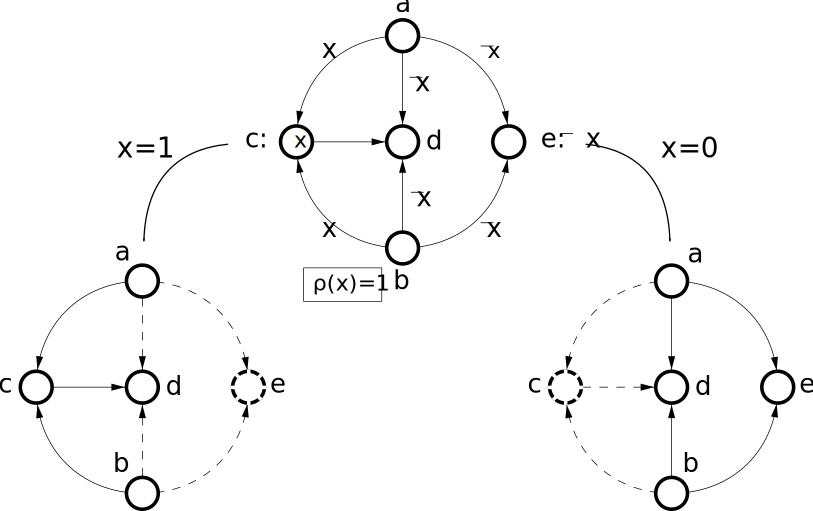
\includegraphics[scale=0.45]{fig/cpog_projections_2}
\par\end{centering}

}
\par\end{centering}

\caption{\label{fig-cpog-examples}Graphical representation of CPOGs and their projections}
\end{figure}


Figure~\ref{fig-cpog-examples}(a) shows an example of a CPOG containing
$|V|=5$ vertices and $|E|=7$ arcs. There is a single operational
variable $x$; the restriction function is $\rho(x)=1$, hence both
opcodes $x=0$ and $x=1$ are allowed. Vertices $\{a,\ b,\ d\}$ have
constant $\phi=1$ conditions and are called \emph{unconditional},
while vertices $\{c,\ e\}$ are \emph{conditional} and have conditions
$\phi(c)=x$ and $\phi(e)=\overline{x}$ respectively. Arcs also fall
into two classes: unconditional (arc $c\rightarrow d$) and conditional
(all the rest). As CPOGs tend to have many unconditional vertices
and arcs we use a simplified notation in which conditions equal to
$1$ are not depicted in the graph. This is demonstrated in Figure~\ref{fig-cpog-examples}(b).

The purpose of conditions $\phi$ is to `switch off' some vertices
and/or arcs in the graph according to the given opcode. This makes
CPOGs capable of specifying multiple partial orders or instructions
(a partial order is a form of behavioural description of an instruction).
Figure~\ref{fig-cpog-examples}(c) shows a graph and its two \emph{projections}.
The leftmost projection is obtained by keeping in the graph only those
vertices and arcs whose conditions evaluate to $1$ after substitution
of the operational variable $x$ with $1$. Hence, vertex $e$ disappears,
because its condition evaluates to $0$: $\phi(e)=\overline{x}=\overline{1}=0$.
Arcs $\{a\rightarrow d,\ a\rightarrow e,\ b\rightarrow d,\ b\rightarrow e\}$
disappear for the same reason. The rightmost projection is obtained
in the same way with the only difference that variable $x$ is set
to $0$. Note also that although the condition of arc $c\rightarrow d$
evaluates to $1$ (in fact it is constant $1$) the arc is still excluded
from the resultant graph because one of the vertices it connects (vertex
$c$) is excluded and obviously an arc cannot appear in a graph without
one of its vertices. Each of the obtained projections can be treated
as a specification of a particular behavioural scenario of the modelled
system. Potentially, a CPOG $H=(V,\ E,\ X,\ \rho,\ \phi)$ can specify
an exponential number of different partial orders of events in $V$
according to one of $2^{|X|}$ different possible opcodes.

A CPOG is \emph{well-defined} if all its projections allowed by
$\rho$ are acyclic. We consider only well-defined CPOGs in this thesis,
because a cyclic projection has no natural execution semantics, in
particular it is not clear which event can be executed first unless
some form of a \textquoteleft{}token\textquoteright{} is introduced
as in the Petri Net model~\cite{2002_cortadella_book}.

To summarise, a CPOG is a structure to represent a set of encoded
partial orders in a compact form. Synthesis and optimisation methods
presented in~\cite{2010_mokhov_ieee} provide a way to obtain such
a representation given a set of partial orders and their opcodes.
For example, the CPOG in Figure~\ref{fig-cpog-examples}(c) can be
synthesised automatically from the two partial orders below it and
the corresponding opcodes $x=1$ and $x=0$. The next section shows
that a particular assignment of opcodes to the partial orders has
a strong impact on the final CPOG, therefore in order to obtain the
most compact CPOG representation one has to search for the best opcode
assignment.

Note that partial orders is not the only formalism for formal specification
of instructions. In particular, there is an alternative approach~\cite{1994_baranov_book}
based on automata, which treats every instruction as a burst-mode
state machine and defines an operation of composition on them. While
benefiting from a direct correspondence between flowcharts of algorithms
and automata, the approach cannot model true concurrency: a set of
causally independent events can only be executed as a `burst' in
the same step/clock cycle. Also, it requires explicit memory to track
the current state of the automaton. We believe that partial orders
are better suited for modelling instruction sets of processing units
built on heterogeneous platforms, i.e. exhibiting both asynchronous
and synchronous interactions~\cite{2011_mokhov_tr}.

